\section{Kurven, Flächen und  Netze}
Die rechnergestützte Beschreibung von Kurven und Flächen ist ein wichtiges Gebiet der Computergrafik.
Es ermöglicht die Berechnung geometrischer und physikalischer  Eigenschaften von Körpern so wie deren graphische Darstellung.
Eine zentrale Rolle spielen hierbei geometrische Objekte, die durch Punkte, Kanten und einfache Flächen, wie zum Beispiel Dreiecke oder Vierecke, beschrieben werden können. Man spricht dann auch entsprechend von Dreicks- bzw. Vierecksnetzen. Häufig sind dabei nicht alle möglichen Konstruktionen zulässig und es hat sich ein Struktur herausgebildet, die für die Computergrafik besonders geeignet ist. Zum einen, weil seine grafische Darstellung besonders schnell und einfach möglich ist und zum anderen, weil viele Berechnungen bestimmte Voraussetzungen benötigen, man denke da zum Beispiel an die Oberfläche oder das Volumen eines Körpers.
Von Bedeutung sind in diesem Kontext auch geeignete Datenstrukturen, mit deren Hilfe sich diese Strukturen und gängige Berechnungen effizient verarbeiten lassen. 
Ein weiterer wichtiger Aspekt ist das generieren und modellieren solcher Strukturen. Hierbei treten häufig sogenannte Interpolationsprobleme auf. Sie entstehen aus dem Wunsch heraus, Kurven und Flächen nur durch die Angabe von Punkten zu generieren. 

\subsection{Polygone, Netze und Elemente der diskreten Geometrie}
\begin{Definition}
Ein geschlossenes Polygon ist ein Paar $P:=(V_P,E_P)$, wobei   
\begin{align*}
E_P := \{e_0, \hdots, e_k \} \subset \mathbb{A}^3,
\end{align*}
eine geordnete Menge von paarweise verschiedenen Punkten, die auch Ecken genannt werden, und   
\begin{align*}
K_P: = \biggl \{(e_0,e_1)  \hdots, (e_{k-1},e_k), (e_k,e_0) \biggr\} \subset \mathbb{A}^3 \times \mathbb{A}^3
\end{align*}
die zugehörige Menge der gerichteten Kanten ist. 
Ist $(e_{l-1},e_l) \in K_p$ eine gerichtete Kante, so bezeichnen wir mit 
\begin{align*}
|(e_{l-1},e_l)| := \overline{e_{l-1}e_l} 
\end{align*}
ihre geometrische Realisierung oder einfach Kante und mit 
\begin{align*}
|P|:= \bigcup_{(e_{l-1},e_l) \in K_P} |(e_{l-1},e_l)|
\end{align*}
 die geometrische Realisierung des Polygons oder geometrisches Polygon.


Ein (geschlossenes) Polygon heißt \textbf{einfach}, falls der Schnitt zweier geometrischer Kanten  entweder leer oder genau ein Punkt aus $V$ ist.
Es heißt \textbf{planar}, falls alle Punkte $e \in V_P$ in einer Ebene liegen.
\end{Definition}


\input{polygon_closed.pdf_t} 

\begin{Definition}
Wir nennen  ein geschlossenes Polygon $P'$ eine \textbf{Nummerrierung} von $P$, falls 
$E_{P'} =E_{P}$ (als Mengen) und
$|P'| = |P|$ ist. 
\end{Definition}


Wie wir gleich sehen werden, definiert die Reihenfolge der Punkte eines einfachen, geschlossenen, planaren Polygons eine Orientierung. Um diesen Sachverhalt präzise definieren zu können, benötigen wir einen Satz, der 
auf den ersten Blick als selbstverständlich erscheint aber rein mathematisch betrachtet tatsächlich schwer zu beweisen ist. Es handelt sich um den Jordanschen Kurvensatz:

\begin{Satz}
Sei $P$ ein einfaches, geschlossenes, planares Polygon und $U$ die Ebene, in der alle seine Punkte liegen. 
Dann unterteilt die geometrische Realisierung $|P|$ die Ebene $U$ in genau zwei Gebiete, ein beschränktes, das das Innere des Polygons genannt wird, und ein unbeschränkte, das das Äußere des Polygons genannt wird.
\end{Satz}

\begin{Definition}
Wir bezeichnen das Innere eines Polygons $P$ mit $|\overset{\circ}{P}|$.
\end{Definition}

Mit Hilfe des Jordanschen Kurvensatzes können wir nun sagen, was die Durchlaufrichtung einer Kante ist und schließlich ob ein Polygon mit oder gegen den Uhrzeigersinn orientiert ist.

\begin{Definition}
Sei $P$ ein einfaches, geschlossenes, planares Polygon. Eine gerichtete Kante $(e_{l-1}, e_l) \in E_P$ hat \textbf{positive Durchlaufrichtung}, falls beim Durchlaufen der  Kante $|(e_{l-1}, e_l)|$ von $e_{l-1}$ nach $e_l$ das innere des Polygons stets rechts von der Kante liegt und \textbf{negative Durchlaufrichtung}, falls es stets links von ihr liegt. 
\end{Definition} 
 
\begin{Definition}
Ein einfaches, geschlossenes, planares Polygon $P$ heißt im Uhrzeigersinn orientiert, falls eine und damit alle gerichteten Kanten positive Durchlaufrichtung haben und entsprechend gegen den Uhrzeigersinn orientiert bei negativer Durchlaufrichtung.  
\end{Definition} 

\input{polygon_orientation.pdf_t}  \\
\input{polygon_orientation_c.pdf_t} 

Netze bestehen nun im wesentlichen aus an den Kanten zusammengeklebten, einfachen, geschlossenen, planaren Polygonen.

\begin{Definition}
Sei $N:= \bigcup P_i$ die Vereinigung endlich vieler, einfacher, geschlossener, planarer Polygone, 
$E_N := \bigcup E_{P_i}$ und $K_N := \bigcup E_{P_i}$ die Vereinigung der Ecken beziehungsweise der Kantenmengen.
Analog zu der Definition eines Polygons definieren wir die geometrischen Realisierungen 
$|K_N| := \bigcup |P_i|$ und $|N| := \bigcup |\overset{\circ}{P_i}| \bigcup |K_N|$
\begin{itemize}
\item Dann heißt $N$ \textbf{Netz}, falls Der Schnitt zweier Polygone entweder leer, ein Punkt in $E_N$ oder eine Kante in $K_N$ ist. 

\item Die Menge aller Kanten, die nur zu einem Polygon gehören, heißt Rand von $N$ und wird mit $\partial N$ bezeichnet.
\item Ein Netz heißt \textbf{geschlossen}, falls es keinen Rand gibt, in Zeichen $\partial N = \emptyset$. 
\item Die Polygone des Netzes werden auch als Facetten bezeichnet.
\end{itemize}
\end{Definition} 


Durch die  Orientierung von Polygonen können wir nun den Begriff der Orientierung und der Orientierbarkeit eines Netzes einführen.

\begin{Definition}
Ein Netz $N$ heißt orientierbar, falls man alle seine Polygone so nummerieren kann, dass jede gemeinsame Kante zweier Polygone jeweils entgegengesetzt gerichtet ist. 
\end{Definition}


\input{surface_orientable.pdf_t}  

\begin{Bemerkung}
Ist eine Fläche orientierbar und nummeriert man die Polygone so, dass benachbarte Kanten entsprechend der Definition immer entgegengesetzt gerichtet sind, so sind entweder alle seine Polygone im oder alle seine Polygone gegen den Uhrzeigersinn orientiert.
\end{Bemerkung}

\begin{figure}[H]
    \centering
    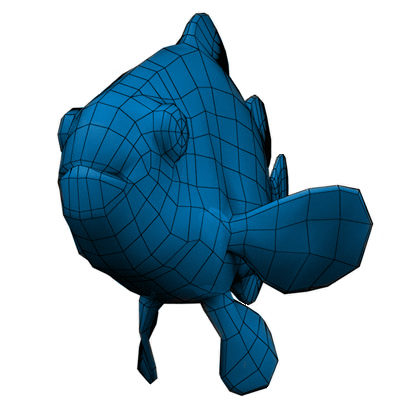
\includegraphics[width=0.4\textwidth]{images/clown_fish.jpg}
    \label{fig:closed-orientable-mesh}
    \caption{Ein geschlossenes, orientierbares Netz. Quelle:CGAL}
\end{figure}

\begin{figure}[H]
\centering
    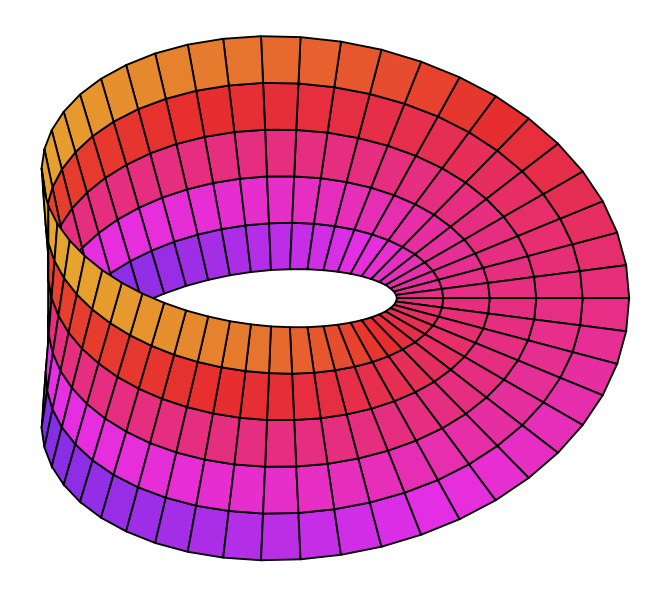
\includegraphics[width=0.4\textwidth]{images/Moebius_strip.png}
    \label{fig:moebius-strip}
    \caption[Möbiusband. Quelle:Wikipedia]{Das sogenannte Möbiusband ist hingegen nicht orientierbar. Es ist nicht geschlossen, sondern hat einen zusammenhängenden Rand. Quelle:Wikipedia}
\end{figure}

\begin{Definition}
Eine Orientierung ist die Wahl einer Klasse von Nummerierungen, so dass alle Polygone entweder im oder gegen den Uhrzeigersinn orientiert sind.
\end{Definition}

\begin{Bemerkung}
Ein Netz hat entweder genau zwei oder keine Orientierung.  
\end{Bemerkung}


\begin{Definition}
Sei $N$ ein orientierbares Netz mit einer Orientierung so gewählt, dass  alle Polygone gegen den Uhrzeigersinn orientiert sind. Wählt man für jedes Polygon $P_i \in N$ drei benachbarte Ecken $e_{j-1}^{P_i}, e_{j}^{P_i}$ und $e_{j+1}^{P_i}$, so erhalten wir
mit $n_{P_i} = e_{j}^{P_i}e_{j+1}^{P_i} \times e_{j}^{P_i}e_{j-1}^{P_i}$ einen Vektor, der Senkrecht auf der Ebene steht in der das Polygon liegt. Wir nennen die Menge $\{P_0, \hdots, P_n\}$ das äußere Normalenfeld des Netzes. 
\end{Definition}


\begin{figure}[H]
    \centering
    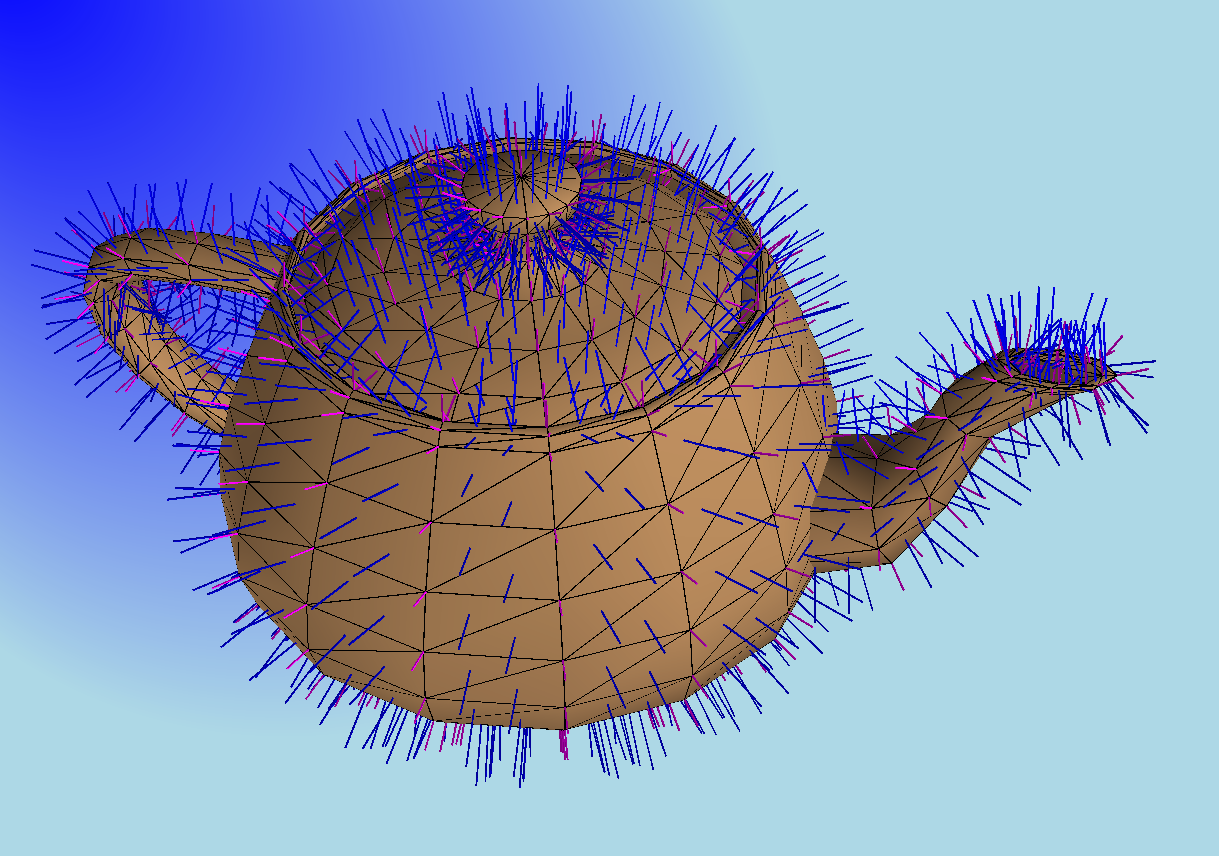
\includegraphics[width=0.7\textwidth]{images/teapot-normals.png}
    \label{fig:outer-normals}
    \caption{Das äußere Normalenfeld}
\end{figure}
Eine wichtige Größe für ein Netz ist die sogenannte Eulercharakteristik, welche in direkter Beziehung zum sogenannten Geschlecht eines Netzes steht.

\begin{Definition}
$N:= \bigcup P_i$ ein Netz. Dann ist die Eulercharacteristig definiert als
\begin{align*}
\chi(N):= \#(E_N) - \#(|K_N|) + \#(N) 
\end{align*}
Sie ist also die Anzahl der  Punkte, minus die Anzahl der geometrischen Kanten, plus die Anzahl der Facetten.
\end{Definition}

Das Geschlecht eines geschlossenen Netzes ist anschaulich gesprochen die Anzahl an Löchern, die durch das geometrische Netz hindurch gehen. Dies lässt sich mit einigem Aufwand mathematisch präzise definieren, jedoch für unsere Zwecke reicht eine Definition durch Beispiele.
\begin{Definition}
Sei $N$ ein geschlossenes Netz. Dann bezeichnen wir mit
\begin{align*}
g(N):= \textbf{Anzahl der Löcher in } |N|
\end{align*}
\end{Definition}
Beispiele:

\begin{figure}[H]
    \centering
    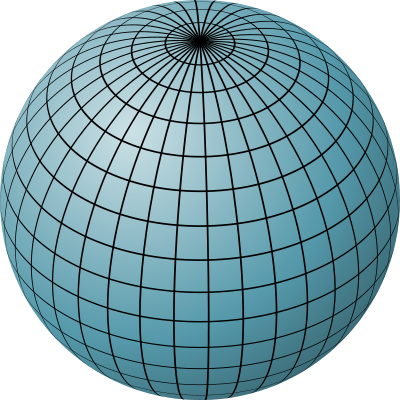
\includegraphics[scale=0.2]{images/Sphere.png}
    \label{fig:closed-mesh-gender0}
    \caption{Geschlossenes Netz vom Geschlecht $0$. Quelle:Wikipedia}
\end{figure}


\begin{figure}[H]
    \centering
    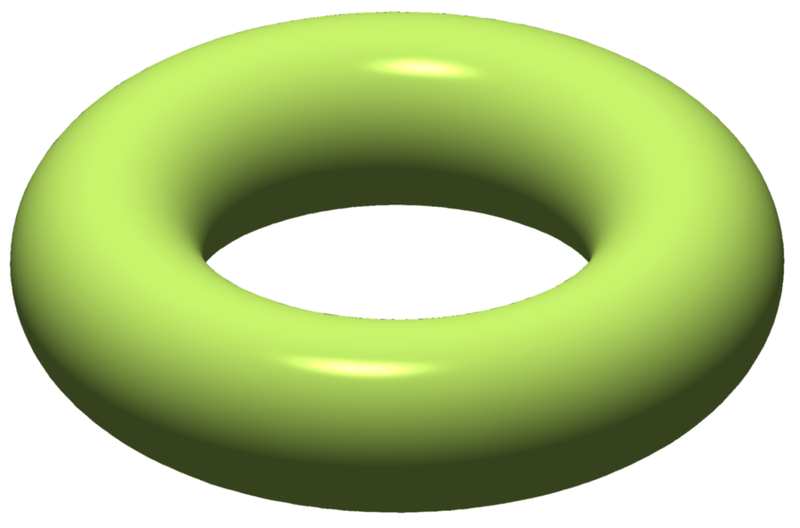
\includegraphics[scale=0.8]{images/Torus.png}
    \label{fig:closed-mesh-gender1}
    \caption{Geschlossenes Netz vom Geschlecht $1$. Quelle:Wikipedia}
\end{figure}


\begin{figure}[H]
    \centering
    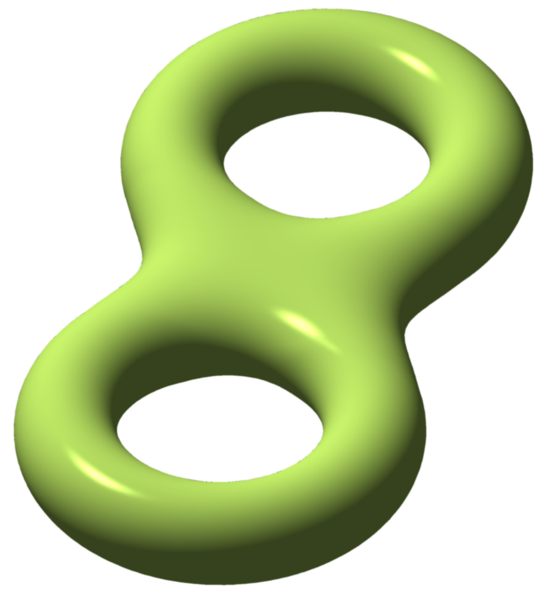
\includegraphics[scale=1.0]{images/Double_torus.png}
    \label{fig:closed-mesh-gender2}
    \caption{Geschlossenes Netz vom Geschlecht $2$. Quelle:Wikipedia}
\end{figure}

\begin{figure}[H]
    \centering
    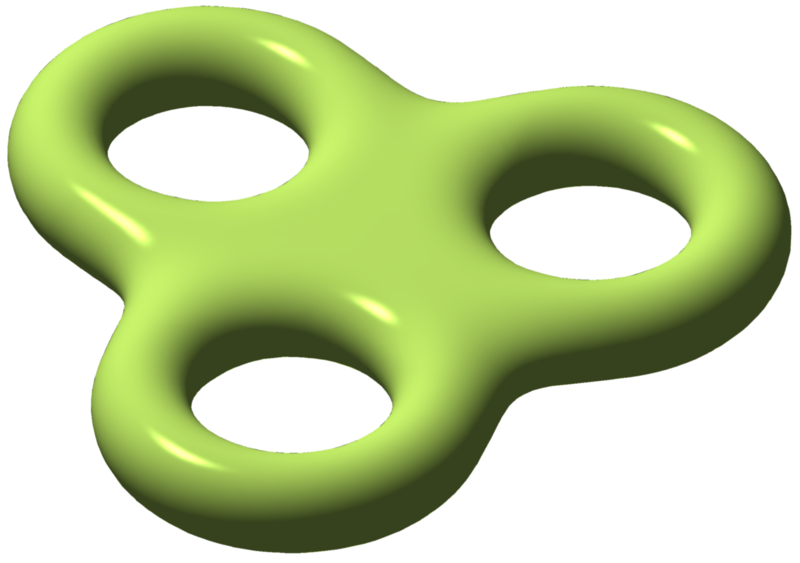
\includegraphics[scale=1.0]{images/Triple_torus.png}
    \label{fig:closed-mesh-gender3}
    \caption{Geschlossenes Netz vom Geschlecht $3$. Quelle:Wikipedia}
\end{figure}

Der Zusammenhang zwischen der Eulercharacteristik und dem Geschlecht wurde im allgemeinen Fall von dem Mathematiker  
Henri Poincare und vorher in einem Spezialfall von Leonard Euler bewiesen. 
\begin{Satz}
Für ein geschlossenes Netz $N$ gilt $\chi(N) = 2 - 2g(N)$. 
\end{Satz}

\begin{Bemerkung}
Nach dem Satz lässt sich das Geschlecht und somit die Anzahl der Löcher via $g(N) = \frac{2- \chi(N)}{2}$ berechnen.
\end{Bemerkung}

\subsection{Datenstrukturen}
\begin{Definition}
Eine Liste ist eine Datenstruktur, in der man Objekte unter Beachtung der 
Reihenfolge speichern kann. 
Für eine Liste von Objekten $O_1,~\hdots,~O_n$ verwenden wir die Notation 
\begin{equation*}
    E = (O_1,~\hdots,~O_n )
\end{equation*}
Jedes Element kennt seinen Vorgänger und Nachfolger und man kann direkt 
auf das $i$-te Element zugreifen:
\begin{equation*}
    %TODO: maybe nicer placement possible here?
    \begin{matrix}
        E[i] & := & O_i \\
        \textrm{prev}(E[i]) & := & O_{i-1} \\
        \textrm{next}(E[i]) & := & O_{i+1} \\
    \end{matrix}
\end{equation*}
Dabei bezeichnet $\textrm{prev}(E[i])$ den Vorgänger und $\textrm{next}(E[i])$ 
den Nachfolger, wobei 
\begin{equation*}
    \forall l \in \mathbb{N} : \{E[l] = \textrm{NULL}~|~(l>n) \vee (l<0)\}
\end{equation*}
$i$ wird auch als Index des $i$-ten Listenelements bezeichnet. 
\end{Definition}

\begin{Definition}[Eckenliste]
In einer Liste $E = (e_1, e_2, \hdots, e_n)$ werden Referenzen auf die Ecken 
gespeichert. 
Eine Referenz im $\mathbb{R}^3$ könnte so aussehen: 
\begin{equation*}
    e_k = \begin{pmatrix}
        x_k \\
        y_k \\
        z_k
    \end{pmatrix}
\end{equation*}
Die $i$-te Facette wird als Liste $F_i = \bigl( i_1,~\hdots,~i_l  \bigr)$ von 
Referenzen auf die Eckenliste gespeichert. 
Die $k$-te Ecke der $i$-ten Facette kann so z.B. mit $E[F_i[k]]$ referenziert 
werden. 
\end{Definition}
\begin{multicols}{2}[Vor- und Nachteile:]
    \begin{itemize}
        \item[+] Einfach zu implementieren
        \item[+] Orientierung kann durch Konvention gespeichert werden
        \item[-] Nachbarschaftsbeziehungen nicht enthalten / schwierig zu 
                 berechnen
        \item[-] Die Zugehörigkeit einer Ecke zu einer Kante muss immer 
                 berechnet werden
        \item[-] Point-in-Mesh fast unmöglich zu berechnen
    \end{itemize}
\end{multicols}

\begin{Definition}[Kantenliste]
In einer Liste $E = (e_1,~e_2,~\hdots,~e_n)$ werden Referenzen auf die Ecken 
gespeichert. 

In einer Liste 
$K = \bigl( (i_{e_1},~\hdots,~i_{e_n}),~
            \hdots,~
            (i_{e_1},~\hdots,~i_{e_m}) \bigr)$ 
werden die Kanten als Tupel von Referenzen auf die Eckenliste abgespeichert. 

Die $k$-te Facette wird als Liste $F_k = \bigl( K[j_1],~\hdots,~K[j_l] \bigr)$ 
von Referenzen auf die Kantenliste gespeichert. 

In einer Liste 
$M = \bigl( (M(i_1),~M(i_2)),~\hdots,~(M(l_1),~M(l_2)) \bigr )$ 
werden die Referenzen auf Facetten in Tupeln abgespeichert, die die 
entsprechende Kante in der Kantenliste als Kante haben. 

$M[i] \in M$ sind also zwei Facetten, die $K[i] \in K$ als Kante haben. 
Der erste Eintrag der Facette befindet sich links und der zweite rechts von der 
Kante. 

Ist die Kante eine Randkante, so wird der andere Wert des Tupels auf $-1$ 
gesetzt. 
\end{Definition}
\begin{multicols}{2}[Vor- und Nachteile:]
    \begin{itemize}
        \item[+] Nachbarschaftsbeziehungen der Polygone werden gespeichert 
        \item[-] Orientierung der Kanten geht verloren (schwierig zu speichern) 
    \end{itemize}
\end{multicols}

\begin{Definition}[Halfedge]
In einer Liste $E = (e_1, e_2, \hdots, e_n)$ werden Referenzen auf die Ecken gespeichert.  Es wird eine Datenstruktur namens Halfedge eingeführt.
Eine Halfedge besitzt eine Referenz auf den Anfangspunkt und auf den Endpunkt. Ebenso besitzt sie Referenzen auf die Gegenüberliegende Kante, bei der der Anfangs und Endpunkt vertauscht ist, sowie eine Referenz auf eine folgende Halfedge  und eine vorangehende Halfedge. Ebenso hält sie eine Referenz auf die Facette, die sie Berandet. Die unendliche Zelle oder äussere Zelle wird wieder  mit $-1$ bezeichnet. Eine Facette ist dann eine Liste mit Referenzen von Halfedges beziehungsweise reicht auch die  Referenz auf eine Halfedge.
\end{Definition}
\begin{multicols}{2}[Vor- und Nachteile:]
    %TODO:
    %\begin{itemize}
        % + Alle kombinatorischen Daten effizient gespeichert (!)
        %    + Orientierung bleibt erhalten
        % - Komplexe Implementierung
        % - Overhead (große Datenmengen)
        % - Nur für orientierbare Netze!
    %\end{itemize}
\end{multicols}

\begin{figure}[H]
    \centering 
    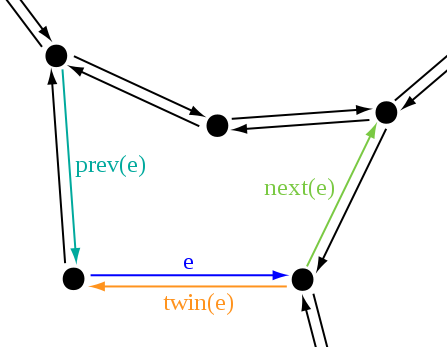
\includegraphics[scale=0.5]{images/halfedge.png}
    \label{fig:halfedge}
    \caption{Halfedge. Quelle :Wikipedia}
\end{figure}

\subsection{Modellierung}

\subsubsection{Parameterdarstellungen}

\begin{Definition}
Eine Kurve ist eine  Abbildung 
\begin{align*}
c: I \subset \mathbb{R} \to \mathbb{R}^3 \\
c(t) := \begin{pmatrix} x(t) \\  y(t) \\ z(t) \end{pmatrix}
\end{align*}
bei der die Funktionen $x, y, z : I \to \mathbb{R}$ stetig sind. Sie heisst differenzierbar, falls $x,y,z$ differenzierbar sind und die Ableitung ist dann definiert als 
\begin{align*}
c': I \subset \mathbb{R} \to \mathbb{R}^3 \\
c'(t) := \begin{pmatrix} x'(t) \\  y'(t) \\ z'(t) \end{pmatrix} \; .
\end{align*}
 \end{Definition}

\begin{Beispiel}
Die Kurve 
$c : [0, 2\pi]  \to  \mathbb{R}^3$, $c(t) :=  \begin{pmatrix} r \cos(t) \\ r  \sin(t) \\  0 \end{pmatrix}$
beschreibt einen Kreis mit Radius $r$, der in der XY-Ebene liegt. Die Ableitung ist
\begin{align*}
c'(t) =  \begin{pmatrix} (r \cos(t))' \\  (r\sin(t))' \\  0 \end{pmatrix} = \begin{pmatrix} -r \sin(t) \\ r \cos(t) \\  0 \end{pmatrix} \;.
\end{align*} 
\end{Beispiel}

\begin{Beispiel}
Die Kurve 
$c :  \mathbb{R}   \to  \mathbb{R}^3$, $c(t) :=  \begin{pmatrix} \cos(t) \\  \sin(t) \\  t \end{pmatrix}$
beschreibt eine sogenannte Helix. Die Ableitung ist
\begin{align*}
c'(t) =  \begin{pmatrix} \cos'(t) \\  \sin'(t) \\  t'  \end{pmatrix} = \begin{pmatrix} -\sin(t) \\  \cos(t) \\  1 \end{pmatrix} \;.
\end{align*} 
\end{Beispiel}
\begin{figure}[H]
    \centering
    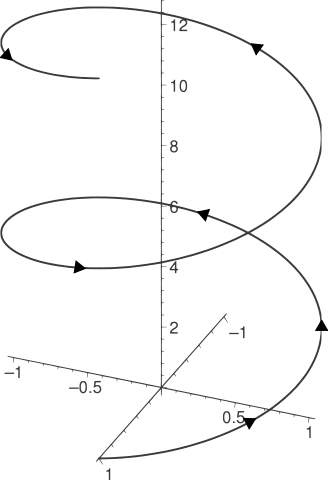
\includegraphics[scale=0.45]{images/Helix.png}
    \label{fig:helix}
    \caption{Eine Helix. Quelle:Wikipedia}
\end{figure}

\begin{Definition}
Ist $c: I \subset \mathbb{R} \to \mathbb{R}^3$ eine stückweise differenzierbare Kurve, so heißt
\begin{align*}
l(c) := \int_{I} ||c'(t)|| dt
\end{align*}
ihre Länge.
\end{Definition}


%\begin{Definition}
%Ein Fläche ist (im wesentlichen)  eine Abbildung
%\begin{align*}
%s: U \subset \mathbb{R}^2 \to \mathbb{R}^3 \\
%s(u,v) := \begin{pmatrix} x(u,v) \\ y(u,v) \\ z(u,v) \end{pmatrix} 
%\end{align*} 
%bei der die Abbildungen $x, y, z : U \subset \mathbb{R}^2 \to \mathbb{R}^3$ stetig sind. Sie heißt differenzierbar, %falls die partiellen Ableitungen
%\begin{align*}
%\frac{\partial}{\partial u} s(u,v) = \begin{pmatrix}  \frac{\partial}{\partial u} x(u,v) \\  \frac{\partial}{\partial u} y(u,v) \\  \frac{\partial}{\partial u} z(u,v) \end{pmatrix}
%\end{align*}
%und 
%\begin{align*}
%\frac{\partial}{\partial v} s(u,v) =  \begin{pmatrix} \frac{\partial}{\partial v} x(u,v) \\ \frac{\partial}{\partial v} y(u,v) \\ \frac{\partial}{\partial v} z(u,v) \end{pmatrix}
%\end{align*}
%existieren. Die Ebene 
%\begin{align*}
%T_s(u,v) :=  \{ s(u,v) + \lambda \cdot \frac{\partial}{\partial u} s(u,v) + \mu \cdot \frac{\partial}{\partial v} \; | \; \lambda, \mu \in \mathbb{R} \}
%\end{align*}
%heißt Tangentialebene am Punkt $(u,v)$ und  der Vektor 
%\begin{align*}
%n (u,v):= \frac{\partial}{\partial u} s(u,v) \times \frac{\partial}{\partial v} s(u,v) \; ,
%\end{align*}
%welcher Senkrecht auf dieser Ebene steht,  die Normale.
%\end{Definition}



\subsubsection{Bezier Kurven}
\begin{Definition}
Die Bernsteinpolynome vom Grad $n$ sind definiert als
\begin{align*}
B_i^n(t) := \begin{pmatrix} n \\ i \end{pmatrix} (1-t)^{n-i}t^i
\end{align*}
mit $i = 0, \hdots n$, $t \in [0,1]$ und dem Binomialkoeffizient
\begin{align*}
\begin{pmatrix} n \\ i \end{pmatrix} := \frac{n!}{i!(n-i)!} = \frac{n(n-1) \cdots 1}{i(i-1) \cdots 1 (n-i) (n-i-1) \cdots 1 } \; .
\end{align*}
\end{Definition}

\begin{figure}[H]
    \centering
    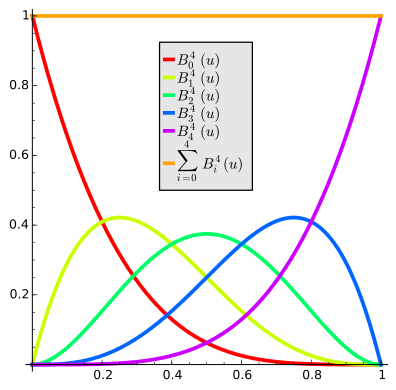
\includegraphics[scale=0.8]{images/Bernstein_Polynomials.png}
    \label{fig:bernstein-polynomial}
    \caption{Die Bernsteinpolynome $B^{4}_i$ und deren Summe. Quelle:Wikipedia}
\end{figure}

\begin{Bemerkung}
Die Bernsteinpolynome vom Grad $n$ bilden eine Basis des Vektorraums der Polynome vom Grad $n$ im Intervall $[0,1]$.
\end{Bemerkung}

\begin{Satz}
Es gilt die Rekursionsformel
\begin{align*}
B_i^n(t) = (1-t) \cdot B^{n-1}_{i}(t) + t \cdot B^{n-1}_{i-1}(t)
\end{align*}
mit $B^0_0(t) = 1$ und $B^i_n(t) = 0$ für $i<0$ oder $i>n$.
\end{Satz}
\begin{proof}
Folgt fast direkt aus der Rekursionsformel des Binomialkoeffizienten
\begin{align*}
\begin{pmatrix} n \\ i \end{pmatrix} = \begin{pmatrix} n-1 \\ i \end{pmatrix} + \begin{pmatrix} n-1 \\ i-1 \end{pmatrix} 
\end{align*}
\begin{figure}[H]
    \centering
    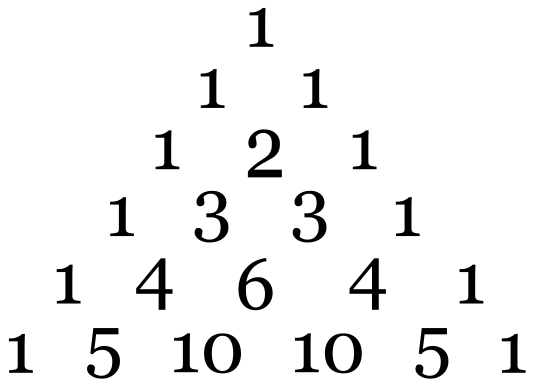
\includegraphics[scale=0.2]{images/pascal.png}
    \label{fig:pascals-triangle}
    \caption{Pascalsches Dreieck}
\end{figure}
\end{proof}


\begin{Definition}
Seien $b_0, \hdots b_n \in \mathbb{R}^3$. Dann heißt die Kurve
\begin{align*}
B^n(t) := \sum_{i = 0}^{n} B_i^n(t) \cdot  b_i \; , t \in [0,1] 
\end{align*} 
eine Bezierkurve vom Grad $n$. Die $b_i$ werden auch Kontrollpunkte genannt.
Für ein beliebiges Intervall $[a,b]$ definieren wir
\begin{align*}
B^n_{[a,b]} (t):=  B^n\biggl( \frac{t-a }{a-b} \biggr) \; , t \in [a,b] \; .
\end{align*} 
\end{Definition}


\begin{Satz}
Eine Bezierkurve hat die Ableitung
\begin{itemize}
\item $(B^n)'(t) = n \cdot \sum_{j = 0}^{n-1} B_{j}^{n-1}(t) \cdot (b_{j+1} - b_j) \; ,$ und nach der Kettenregel
\item $(B^n_{[a,b]})'(t) = \frac{1}{b-a} (B^n)' \bigl(\frac{t -a}{b-a} \bigr)$  für ein beliebiges Parameterintervall.
\end{itemize}
\end{Satz}

\begin{Satz}[Algorithmus von de Casteljau]
Sei $B^n(t) := \sum_{i = 0}^{n} B_i^n(t) \cdot  b_i$ eine Bezierkurve. Für ein 
$t_0 \in [0,1]$ definieren wir rekursiv  
\begin{align*}
b_i^k := \begin{cases}
b_i   & i= 0, \hdots,  n \\
(1-t_0) \cdot b_{i-1}^{k-1} + t_0 \cdot b_{i}^{k-1} &  i = 1, \hdots , n \; \;   k = 1, \hdots , i 
\end{cases} 
\end{align*}
was sich schematisch folgendermaßen darstellen lässt: 
\begin{align*}
\xymatrix{
b_0   \ar@{}[r]|-{=}  &  b_0^0 \ar[dr]^{\cdot(1-t_0)}  &  & & & & & &  \\
b_1   \ar@{}[r]|-{=}  &  b_1^0  \ar[r]^{\cdot t_0} \ar[dr]^{\cdot(1-t_0)} &   b_1^1  \ar[dr]^{\cdot(1-t_0)} & & & & & & \\
b_2   \ar@{}[r]|-{=}  \ar@{..}[d] &  b_2^0  \ar[r]^{\cdot t_0}  \ar@{..}[d] &   b_2^1 \ar[r]^{\cdot t_0}  \ar@{..}[d] &  b_2^2   \ar@{..}[dr]& & & & & \\
b_{n-1}   \ar@{}[r]|-{=}  &  b_{n-1}^0   \ar[r]^{\cdot t_0}  \ar[dr]^{\cdot(1-t_0)} &    b_{n-1}^1   \ar[r]^{\cdot t_0}  \ar[dr]^{\cdot(1-t_0)} &  b_{n-1}^2  \ar@{..}[r] &  
b_{n-1}^{n-1}  \ar[dr]^{\cdot(1-t_0)} & & & & \\
b_{n}   \ar@{}[r]|-{=}  &  b_{n}^0  \ar[r]^{\cdot t_0}  &    b_{n}^1   \ar[r]^{\cdot t_0}  &  b_{n}^2  \ar@{..}[r] & b_{n}^{n-1}   \ar[r]^{\cdot t_0}& b_{n}^{n}& & & 
}
\end{align*}
Dann gilt $b_n^n = B^n(t_0)$.
\end{Satz}

\input{deCasteljau.pdf_t} 



\begin{Definition}[Patching]
Seien $B^n(t)$ und $B^m(t)$  Bezierkurven. Man spricht von eimen $C^0$-patching, falls
 \end{Definition}

\input{bezier_patch.pdf_t} 


\begin{figure}[H]
    \centering
    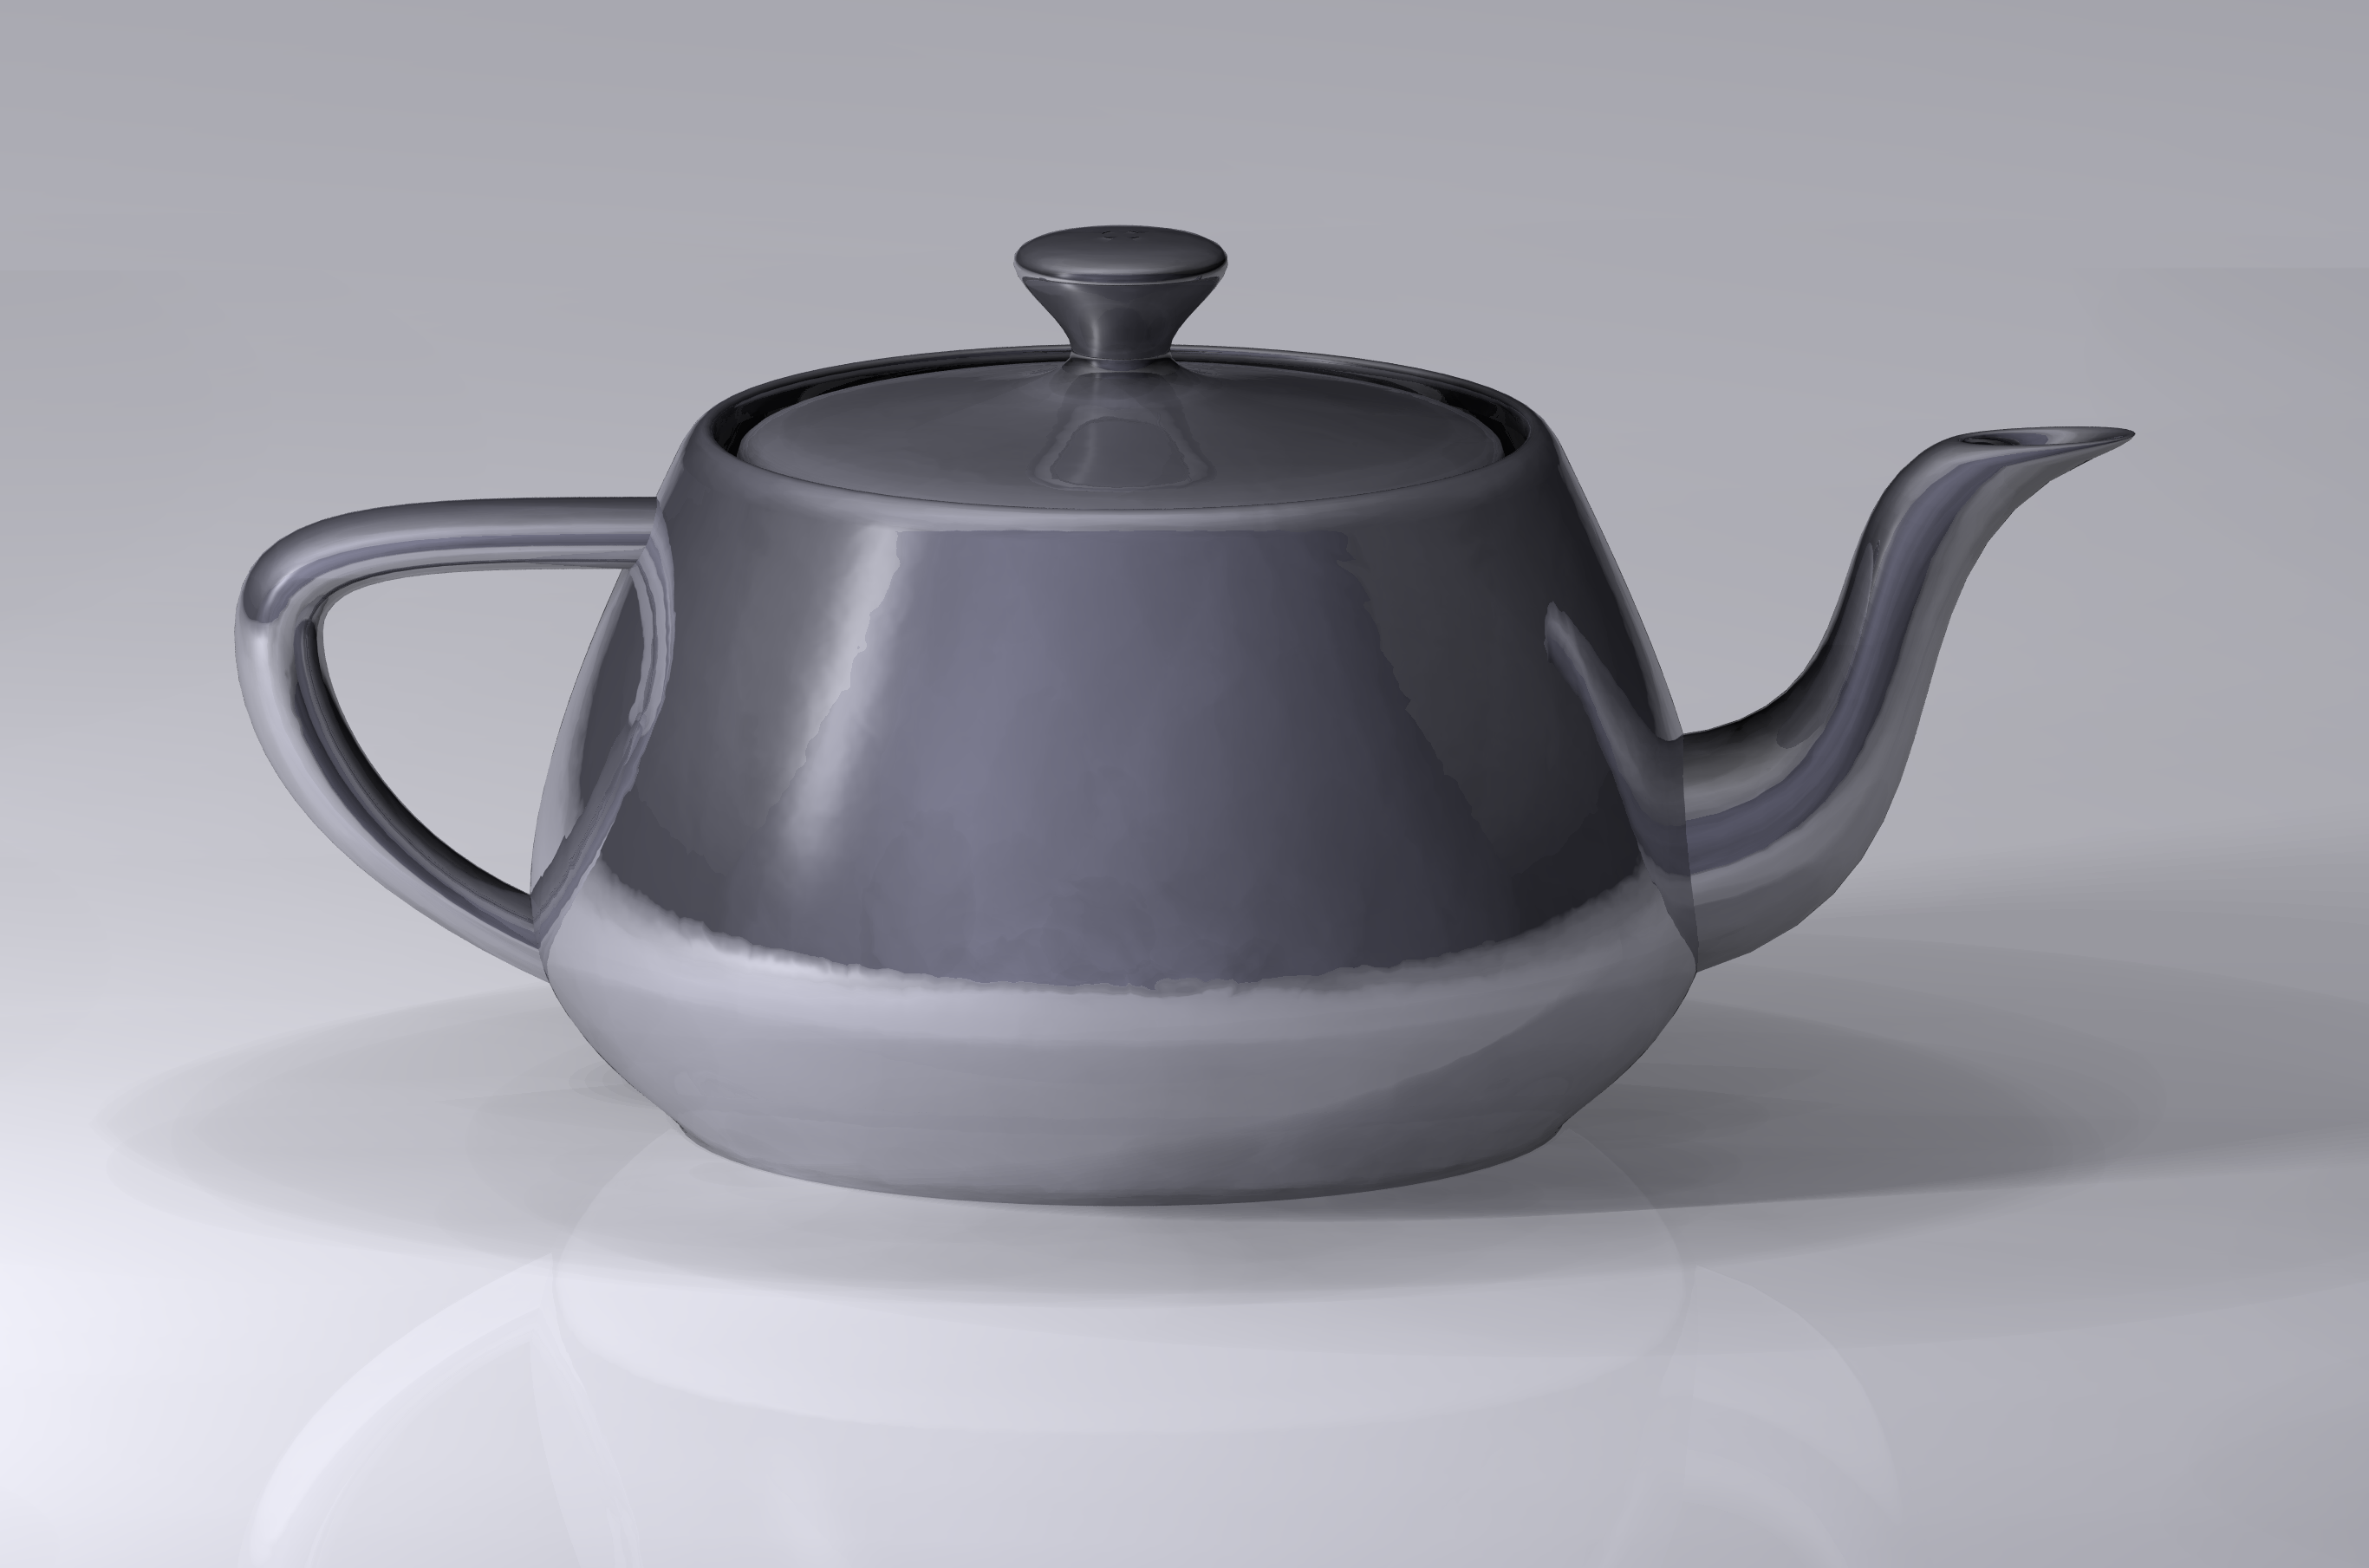
\includegraphics[scale=0.1]{images/Utah_teapot.png}
    \label{fig:rendering-utah-teapot}
    \caption[Ein Rendering der Utah Teekanne]{Ein Rendering der Utah Teekanne, eines der weit verbreitetsten 3D-Modelle in der Computergrafik. Sie wurde mit Bezierflächen modelliert.}
\end{figure}

\subsubsection{Subdivision}


\subsection{Labor}
